%%%%%%%%%%%%%%%%%%%%%%%%%%%%%%%%%%%%%%%%%
% Masters/Doctoral Thesis 
% LaTeX Template
% Version 2.4 (22/11/16)
%
% This template has been downloaded from:
% http://www.LaTeXTemplates.com
%
% Version 2.x major modifications by:
% Vel (vel@latextemplates.com)
%
% This template is based on a template by:
% Steve Gunn (http://users.ecs.soton.ac.uk/srg/softwaretools/document/templates/)
% Sunil Patel (http://www.sunilpatel.co.uk/thesis-template/)
%
% Template license:
% CC BY-NC-SA 3.0 (http://creativecommons.org/licenses/by-nc-sa/3.0/)
%
%%%%%%%%%%%%%%%%%%%%%%%%%%%%%%%%%%%%%%%%%

%----------------------------------------------------------------------------------------
%	PACKAGES AND OTHER DOCUMENT CONFIGURATIONS
%----------------------------------------------------------------------------------------

\documentclass[
11pt, % The default document font size, options: 10pt, 11pt, 12pt
%oneside, % Two side (alternating margins) for binding by default, uncomment to switch to one side
english, % ngerman for German
singlespacing, % Single line spacing, alternatives: onehalfspacing or doublespacing
%draft, % Uncomment to enable draft mode (no pictures, no links, overfull hboxes indicated)
%nolistspacing, % If the document is onehalfspacing or doublespacing, uncomment this to set spacing in lists to single
%liststotoc, % Uncomment to add the list of figures/tables/etc to the table of contents
%toctotoc, % Uncomment to add the main table of contents to the table of contents
%parskip, % Uncomment to add space between paragraphs
%nohyperref, % Uncomment to not load the hyperref package
headsepline, % Uncomment to get a line under the header
%chapterinoneline, % Uncomment to place the chapter title next to the number on one line
%consistentlayout, % Uncomment to change the layout of the declaration, abstract and acknowledgements pages to match the default layout
]{MastersDoctoralThesis} % The class file specifying the document structure

\usepackage[utf8]{inputenc} % Required for inputting international characters
\usepackage[T1]{fontenc} % Output font encoding for international characters

\usepackage{palatino} % Use the Palatino font by default

\usepackage[backend=bibtex,style=numeric,natbib=true]{biblatex} % Use the bibtex backend with the authoryear citation style (which resembles APA)

\addbibresource{bibliography.bib} % The filename of the bibliography

\usepackage[autostyle=true]{csquotes} % Required to generate language-dependent quotes in the bibliography

%----------------------------------------------------------------------------------------
%	MARGIN SETTINGS
%----------------------------------------------------------------------------------------

\geometry{
	paper=a4paper, % Change to letterpaper for US letter
	inner=2.5cm, % Inner margin
	outer=3.8cm, % Outer margin
	bindingoffset=.5cm, % Binding offset
	top=1.5cm, % Top margin
	bottom=1.5cm, % Bottom margin
	%showframe, % Uncomment to show how the type block is set on the page
}

%----------------------------------------------------------------------------------------
%	THESIS INFORMATION
%----------------------------------------------------------------------------------------

\thesistitle{Application of machine learning to temporal point process prediction} % Your thesis title, this is used in the title and abstract, print it elsewhere with \ttitle
\supervisor{Dr. Mark \textsc{Herbster}} % Your supervisor's name, this is used in the title page, print it elsewhere with \supname
\examiner{} % Your examiner's name, this is not currently used anywhere in the template, print it elsewhere with \examname
\degree{Master of Science} % Your degree name, this is used in the title page and abstract, print it elsewhere with \degreename
\author{Badrul \textsc{Alom}} % Your name, this is used in the title page and abstract, print it elsewhere with \authorname
\addresses{} % Your address, this is not currently used anywhere in the template, print it elsewhere with \addressname

\subject{Data Science} % Your subject area, this is not currently used anywhere in the template, print it elsewhere with \subjectname
\keywords{} % Keywords for your thesis, this is not currently used anywhere in the template, print it elsewhere with \keywordnames
\university{\href{http://www.ucl.ac.uk}{University College London}} % Your university's name and URL, this is used in the title page and abstract, print it elsewhere with \univname
\department{Department of Computer Science} % Your department's name and URL, this is used in the title page and abstract, print it elsewhere with \deptname
\group{\href{http://researchgroup.university.com}{Research Group Name}} % Your research group's name and URL, this is used in the title page, print it elsewhere with \groupname
\faculty{\href{http://faculty.university.com}{Faculty Name}} % Your faculty's name and URL, this is used in the title page and abstract, print it elsewhere with \facname

\AtBeginDocument{
\hypersetup{pdftitle=\ttitle} % Set the PDF's title to your title
\hypersetup{pdfauthor=\authorname} % Set the PDF's author to your name
\hypersetup{pdfkeywords=\keywordnames} % Set the PDF's keywords to your keywords
}

\begin{document}

\frontmatter % Use roman page numbering style (i, ii, iii, iv...) for the pre-content pages

\pagestyle{plain} % Default to the plain heading style until the thesis style is called for the body content

%----------------------------------------------------------------------------------------
%	TITLE PAGE
%----------------------------------------------------------------------------------------

\begin{titlepage}
\begin{center}

\vspace*{.06\textheight}
{\scshape\LARGE \univname\par}\vspace{1.5cm} % University name
\textsc{\Large Doctoral Thesis}\\[0.5cm] % Thesis type

\HRule \\[0.4cm] % Horizontal line
{\huge \bfseries \ttitle\par}\vspace{0.4cm} % Thesis title
\HRule \\[1.5cm] % Horizontal line
 
\begin{minipage}[t]{0.4\textwidth}
\begin{flushleft} \large
\emph{Author:}\\
\href{http://www.johnsmith.com}{\authorname} % Author name - remove the \href bracket to remove the link
\end{flushleft}
\end{minipage}
\begin{minipage}[t]{0.4\textwidth}
\begin{flushright} \large
\emph{Supervisor:} \\
{\supname} % Supervisor name - remove the \href bracket to remove the link  
\\
\emph{Advised by:} \\
{Pedro Mediano (Emotech Ltd.)} 
\end{flushright}
\end{minipage}\\[3cm]
 
\vfill

\large \textit{A thesis submitted in fulfillment of the requirements\\ for the degree of \degreename}\\[0.3cm] % University requirement text
\textit{in the}\\[0.4cm]
\deptname\\[2cm] % Research group name and department name
 
\vfill

{\large \today}\\[4cm] % Date
%\includegraphics{Logo} % University/department logo - uncomment to place it
 
\vfill
\end{center}
\end{titlepage}

%----------------------------------------------------------------------------------------
%	DECLARATION PAGE
%----------------------------------------------------------------------------------------

\begin{declaration}
\addchaptertocentry{\authorshipname} % Add the declaration to the table of contents
\noindent I, \authorname, declare that this thesis titled, \enquote{\ttitle} and the work presented in it are my own. I confirm that:

\begin{itemize} 
\item This work was done wholly or mainly while in candidature for a research degree at this University.
\item Where any part of this thesis has previously been submitted for a degree or any other qualification at this University or any other institution, this has been clearly stated.
\item Where I have consulted the published work of others, this is always clearly attributed.
\item Where I have quoted from the work of others, the source is always given. With the exception of such quotations, this thesis is entirely my own work.
\item I have acknowledged all main sources of help.
\item Where the thesis is based on work done by myself jointly with others, I have made clear exactly what was done by others and what I have contributed myself.\\
\end{itemize}
 
\noindent Signed:\\
\rule[0.5em]{25em}{0.5pt} % This prints a line for the signature
 
\noindent Date:\\
\rule[0.5em]{25em}{0.5pt} % This prints a line to write the date
\end{declaration}


%----------------------------------------------------------------------------------------
%	ABSTRACT PAGE
%----------------------------------------------------------------------------------------

\begin{abstract}
\addchaptertocentry{\abstractname} % Add the abstract to the table of contents
While areas of customer recommendation have received a lot of attention in recent years, predicting users behaviour, particularly the timing of their actions, has not had as much focus. The modeling of temporal processes representing human behaviour can be applied across many industries. In this research we examine different methods for predicting a user generated event based on analyzing the timing of their past interactions. Our context is that of music listening and we examine a Bayesian inference model, logistic regression, a linear and RBF SVM, and a RNN-LSTM model. We find that precision and recall pose a trade-off, with a linear SVM being better at the former and an RBF model being better at the latter. We also find that an RNN model achieves relatively good result with a low amount of training data and expect that as computaitonal power improves it will lead to top in class results in this area.

\end{abstract}


%----------------------------------------------------------------------------------------
%	THESIS CONTENT - CHAPTERS
%----------------------------------------------------------------------------------------

\mainmatter % Begin numeric (1,2,3...) page numbering

\pagestyle{thesis} % Return the page headers back to the "thesis" style

% Include the chapters of the thesis as separate files from the Chapters folder
% Uncomment the lines as you write the chapters

% Chapter 1

\chapter{Introduction} % Introduction

\label{Chapter1} % For referencing the chapter elsewhere, use \ref{Chapter1} 

%----------------------------------------------------------------------------------------

% Define some commands to keep the formatting separated from the content 
\newcommand{\keyword}[1]{\textbf{#1}}
\newcommand{\tabhead}[1]{\textbf{#1}}
\newcommand{\code}[1]{\texttt{#1}}
\newcommand{\file}[1]{\texttt{\bfseries#1}}
\newcommand{\option}[1]{\texttt{\itshape#1}}

%----------------------------------------------------------
The modeling of event sequences is useful across industries. For instance the periods in which a customer makes an online purchase can help determine the optimal periods for target marketing. The times at which public transport users tend to travel can help better manage resources to meet demand. The times at which a medical illness re-occurs can help predict future episodes.
 
In all these cases modeling the temporal behaviour of the system is important in predicting the next event. While the area of product recommendation has received extensive attention in recent years, the area of recommendation timing less so. This research looks at how we can model the temporal behaviour of individuals, in order to predice the probability of an event happening at time $t$.

\section{Context}

We take as our context for this research, the goal of estimating the probability that a user of a home-audio device would like to listen to music at a time period $t$, given their play history $h$. One application of this research would be to allow home audio devices to recommend music to a user at an ooportune time. It could then also be extended for other activities.

The goal will be evaluate the effectiveness of several different machine learning methods. The research was guided by Emotech Ltd., a home audio hardware and software company and the creators of Olly \parencite{Olly}.

\section{Data}

The dataset being used in this analysis is the LastFM1k dataset, which is freely available online and contains the listening history of a thousand LastFM listeners. It consists of a series of timestamps denoting when user started played a song. We wish to learn the temporal patterns of a user's behaviour in order to predict the next item in the sequence - a play or non-play event. 

The dataset contains the timestamp, user ID, and track ID of users listening habits over a number of years (2005-2009).

\section{Structure of the report}

We first perform a literature review of 

% Chapter 2

\chapter{Literature Review} % Introduction


\label{Chapter2} % 

Analysing event data presents its own unique challenges and questions. What are the ways to represent the data?  What types of stochastic 
models  are  appropriate  for  explaining  the  structure  in  the  data? How  can  we  measure  
how  well  the  data  is  described  by  a  particular  model?  Within literature the problem is referred to as event prediction, sequence prediction, or temporal point process modelling.

\section{Modelling temporal point processes}

When modelled as a temporal point process, the data can be represented as a sequence of fixed period intervals in one of three ways: as an ordered list of event times ${T_i,...T_n}$, as inter-event times $U_i,...U_n$ where $U_i = T_i-T_{i-1}$, or as a counting process where  $N(t)$ is a count of the number of events occurring before time $t$ \parencite{Borgan}.

\begin{figure}[h!]
	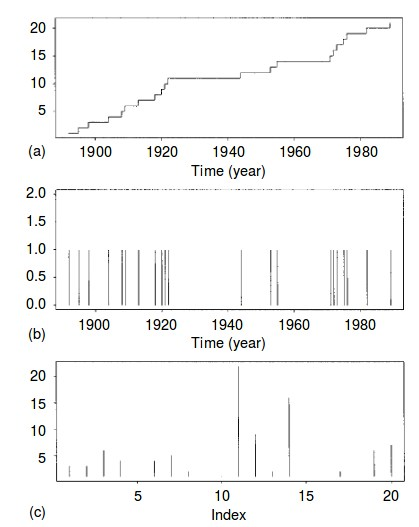
\includegraphics[width=7cm, keepaspectratio]{fig001.jpg}
	\caption{Three different representations of the same point-process a) event count b) date of occurence c) inter-event time}
	\label{fig:fig1}
\end{figure}

Of these, inter-event time is the most commonly used, for example in the times between financial transactions \parencite{EngleRusell}. An example of the counting process is the scoring of goals in soccer \parencite{Heuer}. In the case of music listening, we can model a sequence of events and non-events, where $t_i$ can either be 0 (did not play music) or 1 (played music). This is the form we use in all but the Bayesian model as described in the next chapter.

\newpage

\subsection{Poisson Process}
The Poisson process \parencite{Kingman} is one of the most widely used counting processes. It is a simple point process in which the probability of an event at time $t$ is assumed to be independent from all other times, and where the probability function follows a Poisson distribution with parameter $\lambda$. 

The Poisson process has been used to model:

\begin{itemize}
	\item the number of car accidents at a site or in an area \parencite{venezian};
	\item the location of users in a wireless network \parencite{blaszczyszyn}
	\item customer purchases \parencite{Ehrenberg}
	\item jumps in asset prices  \parencite{kirch}
\end{itemize}

\subsection{Hawkes Process}
In the Poisson process the probability at time $t$ is dependent on time $t$ only. In other types of point process models the probability is dependent on periods prior to $t$ as well, such as the self-exciting (Hawkes) process where the intensity is determined by previous events through the parametric form $\lambda(t) = \mu + \beta \sum_{t_i<t}g(t-t_i)$ and where $g$ is a non-negative kernel function.

The Hawkes process is particularly useful in systems with rapid changes to rate of events and is used a lot in finance to model the intensity of the arrival of trades \parencite{hardiman2013critical}

\subsubsection{Conditional Intensity Function}
The probability function used in a temporal point process is more formally known as a conditional intensity function. It represents the infinitesimal rate at which events are expected to occur around a particular time $t$, conditional on the prior history of the point process prior to time $t$. 
 
If the conditional intensity remains constant over time it is referred to as a homogeneous or stationary point process \parencite{Nok}. If however it can vary with time it is inhomogeneous. 

Note that the logit function used in generalized linear model, can also be thought of a conditional intensity function and has been used to develop sophisticated models such as \parencite{baddeley2014logistic} and \parencite{rajala2014note}.

However, as noted by Wass et. al \parencite{Wass}, point process models using a conditional intensity function often make various parametric assumptions about the latent dynamics governing the generation of the observed point patterns. As a consequence, model misspecification can cause significantly degraded performance in point process models.

\section{Deep Learning}

In recent years deep learning has demonstrated the power to learn hierarchical non-linear patterns on large-scale datasets \parencite{DL} through multiple layers of abstraction (e.g. multi-layer feedforward neural networks). It has achieved state-of-the-art performances on a wide range of applications, such as computer vision \parencite{ImageNet}, natural language processing \parencite{Socher}, and protein structure prediction \parencite{Lena}.

However it has not been applied to temporal point processes until recently with Xiao et. al \parencite{Wass} applying Generative Adversarial Networks (GANS) to the problem. GANs consist of two neural network models - a generator tasked with generating (i.e. predicting) a future sequence of events based on the history, and a discriminator tasked with detecting the true (ground truth) sequence amongst the generated ones.

For measuring the loss between a generated and true sequence, the authors found the Wassertein-Distance \parencite{WassGAN} performed better than Maximum Likihood Estimate (MLE) which they remarked "may suffer from mode dropping or get stuck in an inferior local minimum".

Their findings showed that while parametric point process models work better with problems where a parametetric form exists, with real world data a GAN model with Wasserterin-Distance outperforms all other models. 

\subsection{Recurrent Neural Networks (RNN)}

RNNs are a type of artificial neural network designed to recognize patterns in sequences of data, such as text, genomes, handwriting, the spoken word, or numerical times series data emanating from sensors, stock markets and government agencies. Whilst a traditional Feed-Forward network \parencite{MLP} has input nodes, hidden layers, and an output layer, with data flowing in one direction only, RNNs allow for the hidden state from one timestep of the neural net to be an input into the next (see fig. \ref{RNN}).

\begin{figure}[h!]
	\centering
	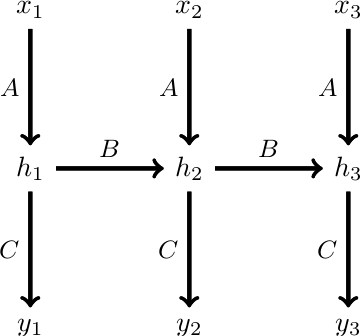
\includegraphics[width=5cm, keepaspectratio,]{fig007.jpg}
	\caption{RNN with 3 timesteps}
	\label{RNN}
\end{figure} 

\subsubsection{LSTM}
RNN models can employ different methods for the propogration of the hidden state over time. One such well known method is Long Short-Term memory (LSTM) \parencite{Olah}. Here the hidden state is the product of a further four layers that interact in a way as to learn what information to retain and what information to throw away. 

\begin{figure}[h!]
	\centering
	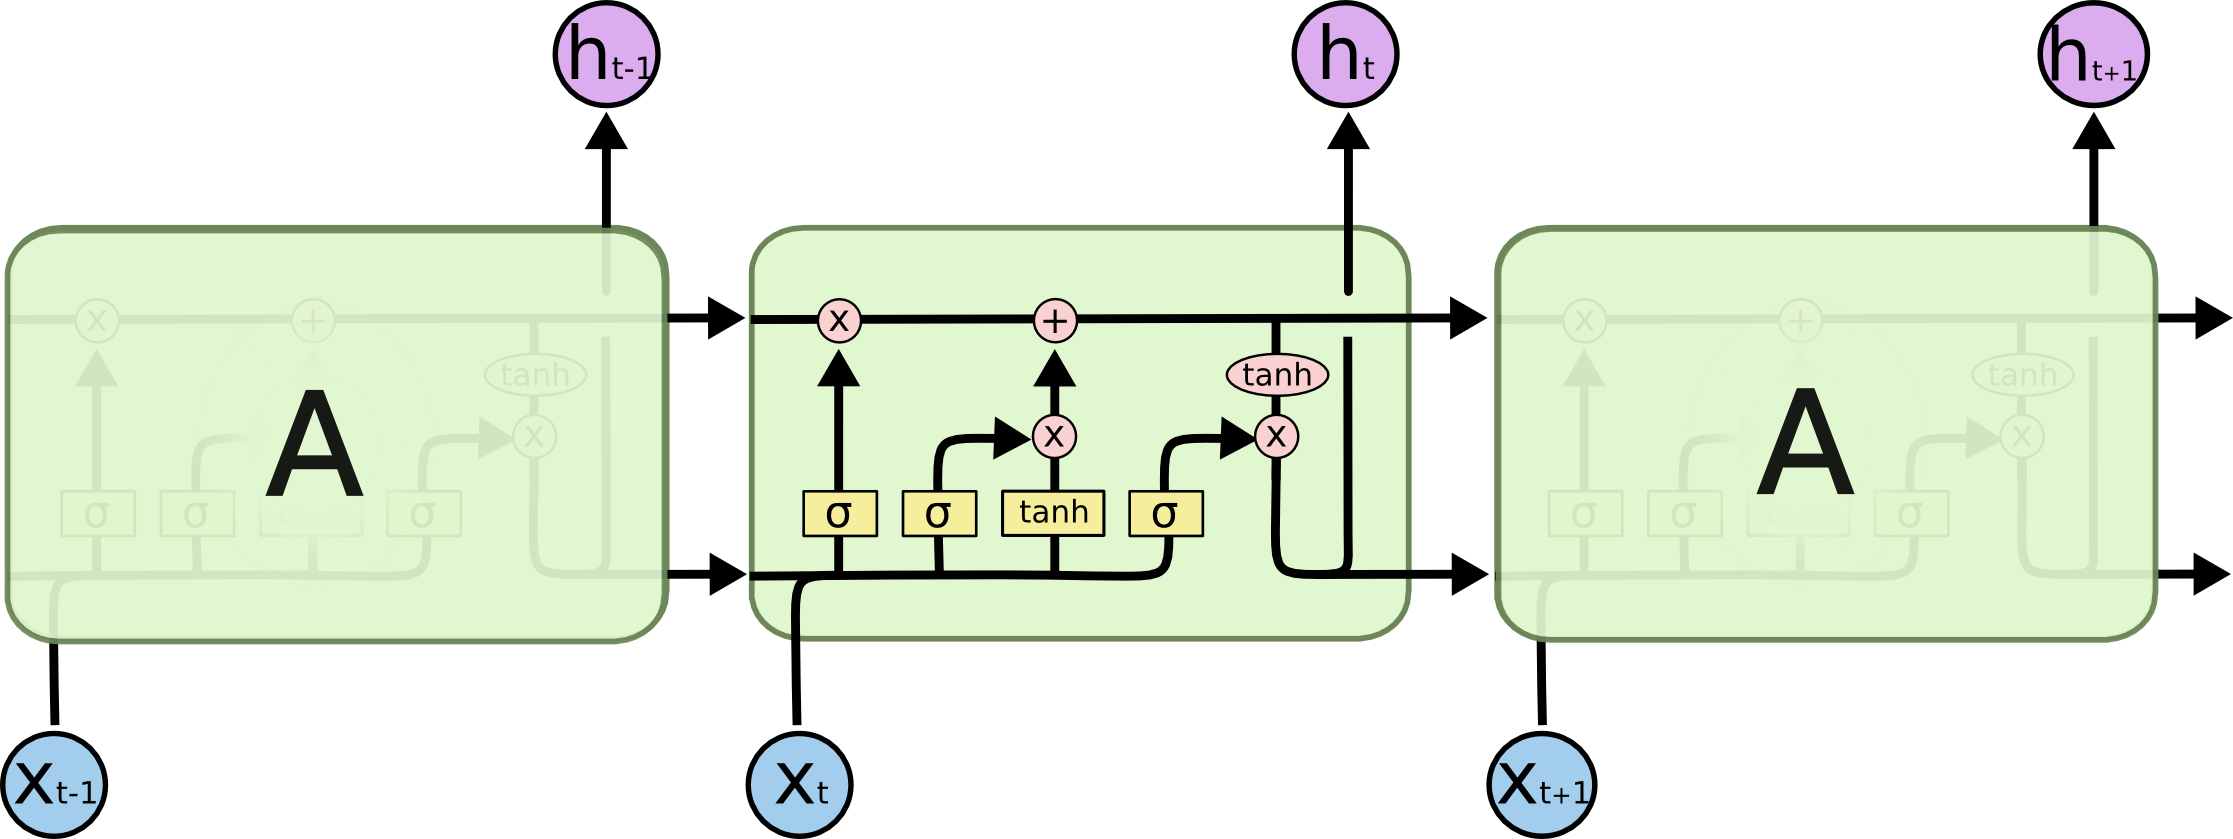
\includegraphics[width=12cm, keepaspectratio,]{fig008.png}
	\caption{LSTM}
	\label{fig:fig8}
\end{figure} 

Malhotra  \parencite{malhotra2015long} demonstrates that LSTMs with 2 layers can learn higher level temporal patterns without prior knowledge of the pattern duration, while more recently \parencite{xiao2017modeling} attempts have been made to combine concepts of temporal point processes with that of an RNN. Here the authors viewed the conditional intensity function of a point process as a non-linear mapping between the predicted transient occurrence intensity of events with different types, and the  model  input  information  of  event  participators, event
profile and the system history.

They model this non-linear mapping by utilizing two RNNs: one for modelling the time-series data and associated features and a second to model long-range dependency over history with arbitrary time intervals; specifically a sequence of event type and the time since the previous event. In this way they can capture both the temporal based patterns, as well as the non-temporal, event-correlations which approximates to a conditional intensity function based on inter-event time.

The favoured evaluation metrics in their research were precision, recall, f1 score, and a confusion matrix, with a logistic regression model used as a baseline to compare against.

\section{Summary}

While not an exhaustive review of techniques we have seen some of the ways in which point processes can be modelled using traditional conditional intensity based models, as well as more recent areas of experimentation using deep learning. In the next chapter we layout the approach and methods we wish to explore in the context of this research. 
% Chapter 3

\chapter{Experimental Design}

\label{Chapter4} % 

In this chapter we describe the different methods that were assessed. The methods, in order of gradually increasing sophistication, are as follows:

\begin{enumerate}
    \item Baseline model
	\item Bayesian Inference
	\item Binary Logistic Regression
	\item Linear SVM Classifier
	\item Non-Linear SVM Classifier
	\item Recurrent Neural Networks
\end{enumerate}

All methods, except for the Bayesian Inference method, require the data to be structured as a time-series. The Bayesian method adopts a different approach that requires the data to be aggregated into half-hourly buckets of a week. The data preparation that was performed is described in the next section, followed by an explanation each method, and the evaluaion criteria for assessing the methods in the sections that follow.

\section{Data preparation}

\subsection{Data transformation}

The analysis was carried out in Python (via Jupyter notebooks) running on Ubuntu. The raw data consisted of timestamps of when a song was played and a user ID. These were loaded as-is into a SqlLite3 database in order to reduce the need to repeat data preparation steps. The methods themselves utilized Scikit-learn for all models, save for the RNN model which used Tensorflow.

UserIDs were converted to integer (e.g. 'User0005' became '5') and a period lookup table was created at $n$ minute intervals, against which all timestamps in our main dataset were mapped to. $n$ was chosen to be a period of 30 minutes.

The data, which contained entries for the times at which each user listened to music, was supplemented with all the times they did \emph{not} listen to music, between their date of their first and last play.  This was required in order to generate a sequence of play and non-play events. 

\subsection{Feature selection}

The features that were chosen were based on the preliminary analysis (see next chapter) and consisted of time-seried and non-time series features. The time-series features were binary, representing play (1) or non-play (0) events at $t, t-1, t-2, t-3, t-4, t-5,  t-12hrs, t-23.5hrs, t-24hrs, t-24.5hrs, t-1wk, t-2wks, t-3wks$, and $t-4wks$.

$t-1$ to $t-5$ represent user activity in the previous 2.5 hours. The remaining time-lags were chosen to represent half-day, daily, and weekly cycles, with additional empahsis around the -24 hour mark due to the daily patterns observed in the preliminary analsysis.  

The non-time lag features were binary features representing the day of the week (isMon, isTue etc.) and the number of hours away from 5pm in either direction - so a timestamp at 4pm and 6pm would both be 1. Again this was based on the observations in the preliminary analysis of 5pm being a peak listening hour.

\section{Validation and Test dataset selection}

Our working dataset was a subset of the full 1000 user dataset, and comprised of 4,217,228 rows of training data across 97 users. Of this a random sample of 100,000 rows was taken and 5-fold cross-validation emplyoyed.  

\subsubsection{Data Imbalance}

A data imbalance is when the training data is when one or more of the classes is under-represented in the dataset. Of the 4,217,228 rows in our working data set, 361,081 (8.6\%) were play events and 91.4\% were non-play events. This can result in models that achieve a high accuracy score by following either of the following two heuristcs:

\begin{itemize}
	\item Predict non-event for everything
	\item Predict $t$ will be the same as $t-1$
\end{itemize}
 
There are several methods for dealing with data imbalance \parencite{Brownlee} including restricting input data, having a weighted loss function, and using recall as an evaluation measure. We used recall as well as weighting. Both class weights and sample weights were employed in the scikit learn models. The class weights were inversely proportional to play \& non-play frequencies in the input data, while the sample weights were a hyper-parameter.  In the RNN model only sample weighting was used.

The effect of class weighting is to encourage the model to predict play events. The effect of the sample weighting is to encourage the model to predict play events while minimizing the number of false-positives.

\section{Methods}

\subsection{Baseline Model}

Our baseline model will be to assume $t = t-1$. That is to say a person will listen to music at period $t$ if, and only if, they listened to music in the period immediately priod. As music listening events tend to be clustered (people listen to music in batches) the accuracy of the baseline model is will be fairly high. However it will not be able to predict the first play of a listening session, or where the listening session duration lasts no longer than a single periodm, which in the experiments is defined as a 30 minute period.

\subsection{Bayesian Inference}

Here we employ a simple Bayesian Inference approach by utilizing the Beta-Binomial model. The Beta-Binomial model is built upon the weekly patterns observed in the preliminary analysis. Conceptually it seeks to build up a users personalized weekly listening profile using a Beta-Binomial probability distribution. The priors for which are based on the population as a whole, and the observations are history $T_h$. We then assess how effective this profile is at predicting listening outcome at time $t$ for that user.

Prior probabilities were calculated for each half-hourly period in a week (24*2*7=336 timeslots). Fig \ref{fig10b} shows the calculations for the first 2.5 hours of a Sunday (d-hour-hh format). 

\begin{figure}[h!]
	\centering
	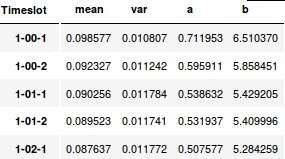
\includegraphics[width=5cm, keepaspectratio,]{fig010b.jpg}
	\caption{}
	\label{fig10b}
\end{figure} 

The liklihood function which represents the probability of a user listening to music was defined as a binomial distribution, where $k$ is the number of plays in a given period, $n$ is the sum of plays and non-plays, and $\theta$ is the unknown probability parameter for the binomial distribution.

$${n \choose k}\,p^{k}(1-p)^{n-k}$$

As the Beta distribution is a conjugate prior to the Binomial the model can be reduced to: $Beta(\alpha+P, \beta+Q)$ where P is the count of plays and Q is the count of non-plays. For which the parameters $\alpha$ and $\beta$, are derived from the training set, with an estimate of the mean for each half-hourly time period as shown in fig \ref{fig10b}. To do this we first calculate the probability of a play (total plays in period / count of plays and non-plays) per user, then take the mean and variance across users. $a$ and $b$ are then determined as:
$a = (\frac{(1- \mu)}{\sigma} - \frac{1}{\mu}) \mu^2$
and
$\beta=\alpha\left(\frac{1}{\mu}-1\right)$.

Finally we convert the probabilites into a binary outcome by optimizing for a threshold $\lambda$ at which we predict a play event.

\subsection{Binary Logistic Regression}

This method (and the subsequent methods) adopts a more classicial time-series approach to the prediction problem by constructing a dataset as a sequence of play events at time $T_t = 1$ and non-play events $T_t = 0$, with $t$ representing a time period of a fixed interval of 30 minute chunks.

\begin{figure}[h!]
	\centering
	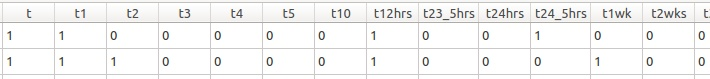
\includegraphics[width=12cm, keepaspectratio,]{fig021.jpg}
	\caption{Example of times-series data}
	\label{fig021}
\end{figure} 

We seek to model the probability of an event in the current time period $t$, given the history of events: $p(Y_t =1 \mid Y_h)$. Our binary logistic model is therefore defined as:
$$p(Y_t = 1|Y_h) = \sigma(w^Tx + b)$$
$$p(Y_t = 1|Y_h) = 1 - p(Y_t = 1|Y_h)$$

with $\sigma$ being the sigmoid function defined as:
$$\sigma(x)=\frac{e^x}{1+e^x}$$

Determining the optimal weights and constant can be determined by maximization of the log-liklihood or the minimization of the negative log-liklihood. 

In addition we will be using an L2 regularizer term,  $ + 1/2w^Tw$, to prevent over-fitting:

\subsection{Linear SVM Classifier}

SVM models work by determining a separation plane between classes based on the support vectors - the data points closes to the decision boundary. A linear SVM regression model performs this through the Epsilon Intesive loss function \parencite{Vapnik}. The objective becomes to \textit{minimize:}

$$max(0,\left\| (y_i - w_i x_i - b) - \epsilon \right\|)$$

In other words we ignore cost functions that are within a certain margin  $\epsilon$. In our case this may be of importance in cases where the probability of user listening to music is close to the decision boundary, which may be the case for the very first song played at the start of a session.

\subsection{RBF SVM Classifier}

Here we use a Gaussian RBF kernel in our SVM model. A Gaussian kernel is a popular method for modeling non-linear decision boundaries. Our model becomes:

$$p(E=1)=b+\sum^N_{i=1}w_iRBF(x,x_i)$$

where the RBF kernel is defined as:

$$K(\mathbf {x} ,\mathbf {x'} )=\exp \left(-{\frac {\|\mathbf {x} -\mathbf {x'} \|^{2}}{2\sigma ^{2}}}\right)$$

Note that actual implementations of this make use of more computationally efficient methods \parencite{TFCookbook}. This restated method has a hyper-parameter $\gamma$ that takes the place of $2\sigma^2$.

\subsection{RNN-LSTM model}

The construction of the RNN model requires a number of hyper-parameters. These are as follows:

\begin{list}{-}
\item Time-steps: How many time steps to use (= batch depth)
\item - Learning rate: Learning rate of backprop algorithm
\item Hidden units: Number of units per hidden layer
	\item Layers: Number of hidden layers
	\item SampleWeighting: Weighting to apply in the cost function for labels that are a play event
	\item User iteration: How many random users to select for training)
	\item SamplesPerUser: How many mini-batches to select for each user
	\item BatchRows: How many random periods to select in each mini-batch (=batch height)
	\item Batch iterations: How many iterations to perform on one batch
\end{list}

\subsubsection{Batch shape}

We provide the RNN model with a sequence of historical data at times $t-1 .. t-n$ with $n >1)$. This is fed into the RNN as separate time steps in forward temporal order (earliest time-steps are processed first). The hidden state would propogate information forward at each time step, until it was used to predict the outcome at time $t$.

Practically speaking this meant feeding in the data with input shape (batch rows, time-steps, features). Some points of interest are:

\begin{enumerate}
	\item The features dimension here only contains $t-1$ and no other feature. 
		
	\item The time-steps are 'unrolled' within Tensorflow and fed into the LSTM. In this research we experiment with different lengths of time-steps, with 48 (half-hour periods ) representing a day, 336 for a week, and 672 for 2 weeks.

	\item When the data is unrolled, time step $t$ for all rows in the batches are processed together as one block, before moving onto the next time-step.

	\item Constructing the 3-d shape often requires building them up in slices. A significant speed up was observed in Python when using a pre-allocated array vs. appending to it.
\end{enumerate}

\subsubsection{Samples and iterations}

A challenge in testing the RNN model was to balance the number of users being samples from, with the number of samples to take from each user, and the numebr iterations to then do on each sample. A distinction between batch rows and samples per user was required for computational reasons to reduce the demand on RAM per mini-batch, vs. feeding in one large mini-batch per user.

\subsubsection{Cost function and weighting}

Both the logistic loss and a weighted softmax cross entropy loss function were tried in the model (the latter requires converting the output label into one-hot encoding format). Logistic loss was found to be the more effective of the two cost function and hence used for our results. 

Secondly due to the imbalanced data, adding weighting to the costs of a Play event was found to be crucial in getting good results. The key snippet of code for the cost function is given below:

\begin{lstlisting}
_logits = RNN(x, weights, biases,n_steps)
_prob = tf.sigmoid(_logits)
_weightstf.add(1,tf.multiply( _
tf.cast(tf.equal(y,1),'int32'),n_weighting))

_logloss =
tf.losses.log_loss(predictions=_prob, _ labels=y,epsilon=0.00001, _ 
weights=_weights)

_cost = tf.reduce_mean(_logloss)
\end{lstlisting}


\section{Evaluation critera}

Deciding on an approporiate evaluation measure requires careful consideration to the costs attached to different predictions. In our case the cost of suggesting music when the user is likely not interested is higher than not playing music when they are likely to be interested. 

A number of possible evaluation criteria were looked at. The most-straight forward of which was \textit{accuracy}. This computes the count of correct predictions as a fraction of the total number of predictions. While this is an intuitive measure, it would not distinguish between models that had a high accuracy on the play-events vs. a high accuracy on non-play events. 

To do this we look at precision. Precision (P) is defined as the number of true positives over the number of true positives plus the number of false positives. A positive in this case is a play-event so our precision equation becomes:

$$Precision = \frac{Correct Play Predictions}{Total Play Predictions}$$. 

This will be measuring our models on how many of the 'Play' events predicted were correct. However it does not distinguish between models that predict a play event only on 'safe bets', such as when t-1 was also a play event, vs. those that are attempting to guess the start of a play sequence. For this we turn to recall.

Recall is defined as:

$$Recall = \frac{CorrectPlayPredictions}{TotalPlayPrectionsInDataset}$$

For example if we predicted 100 plays correctly but there were in fact 110 plays in the dataset, then recall would be 100/(100 + 10)= 91%.


\section{Summary}

We have described how our data was transformed to make it useful for our experiments. In particular how we had to convert our list of play events into a list of play and non-play events for every period. By doing this we are faced with an imbalance of data as non-play events make up ~91\% of the data and so we employ a weighting strategy to counteract this.

We then described the methods we will be utilizing in our experiments, consisting of a Baseline model which simply assumes $t =t-1$, a Bayesian model which builds up a weekly profile of listening habits for each user, Logistic and SVM models that apply classical machine learning techniques to our time-series problem, and finally a deep learning model in the form of an RNN-LSTM where we seek to utilize its ability to learn temporal patterns through a hidden memory state.

Finally we looked at different ways for measuring the success of our problem, with precision and recall being the preferred choice.

In the next chapter we shall present the results of our experiements together with insights on each model.
% Chapter 4

\chapter{Results}

\label{Chapter4}

We begin our discussion of the results with preliminary analysis of the data that helped shape the experimental design. Here we seek to understand what are some of the overarching patterns in music listening habits and how these look at an individual level.

After this we present a summary of our results followed by a discussion of the performance of each individual method.

\section{Preliminary analysis}

\subsection{Daily play patterns}

By grouping track plays into 30 min intervals and aggregating by periods within a day, we see a clear daily pattern with music listening hitting a peak at around 5pm and a trough at around 6am.

\begin{figure}[h!]
	\centering
	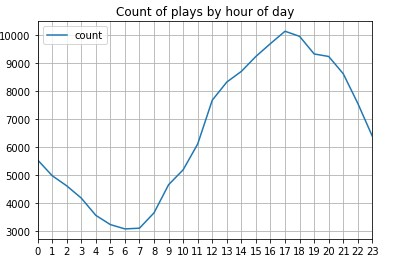
\includegraphics[width=7cm, keepaspectratio,]{fig004.jpg}
	\caption{5-5.30pm is peak listening time}
	\label{3a}
\end{figure} 

Zooming out to view the pattern across an entire week in figure \ref{3b}, we see that the daily pattern occurs across every day of the week with weekends having a lower total number of plays.

\begin{figure}[h!]
	\centering
	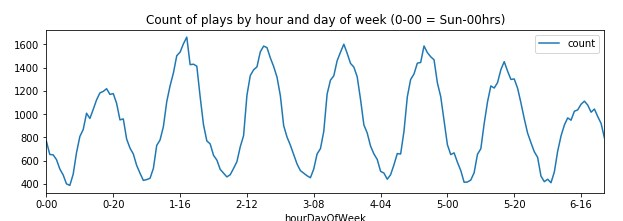
\includegraphics[width=7cm, keepaspectratio,]{fig005.jpg}
	\caption{Most popular times to listen to music across all users}
	\label{3b}
\end{figure} 

At a high level therefore one can get good accuracy by simply anticipating music demand to peak at 5pm. However if we select two users at random, we see (see fig. \ref{3c}) that these daily patters are not as strongly discernable. This demonstrates why models modeling the high levels patterns is not enough for individual user prediction. 

\begin{figure}[h!]
	\centering
	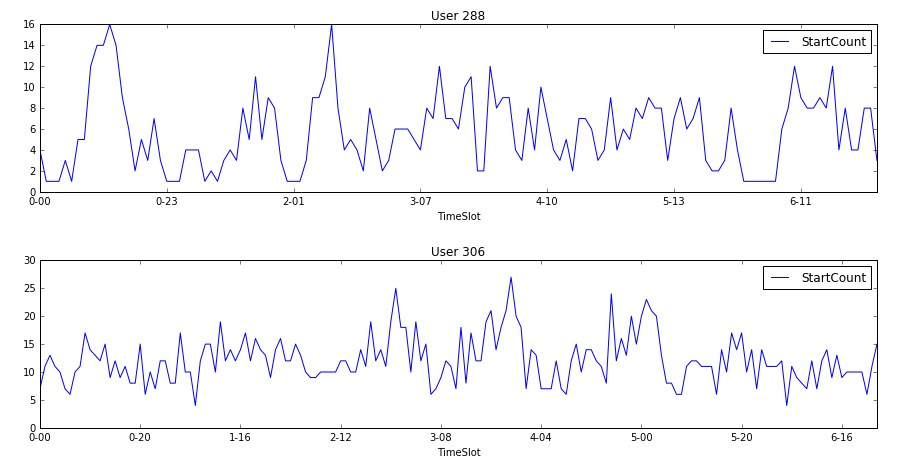
\includegraphics[width=7cm, keepaspectratio,]{fig006.jpg}
	\caption{Most popular times to listen to music by individual user}
	\label{3c}
\end{figure} 

\subsection{Inter-event times}

The dataset contains a timestamp associated with each user. This does not necessarily mean the user played a song in its entirety. Analysis shows plenty of cases where the interval time between tracks was a few seconds suggesting the user skipped tracks. 

Figure \ref{3d} shows a frequency plot of intervals. Intervals beyond 30 minutes continue the exponential decrease and are not shown. We see that while the mode is on par with a typical song length, there is a significant number of plays that lasted under 5 minutes. 

\subsection{Time-series analysis}

Here we examine our data once it has been transformed in a binary sequence of events (1) and non-events(0). We seek to understand better how an optimizer may perform based on traits of the data.

We begin with assessing how well our baseline model may perform based on assuming $t = t-1$. Fig \ref{fig12} shows that the 76\% of Plays, also had a play in t-1. However simply using this as a rule would also capture 2.2\% of non-plays.

\begin{figure}[h!]
	\centering
	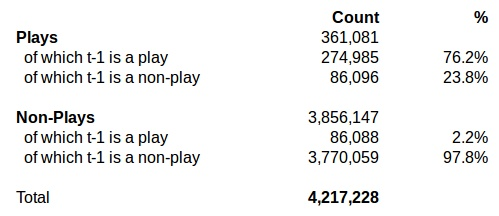
\includegraphics[width=7cm, keepaspectratio,]{fig012.jpg}
	\caption{}
	\label{fig12}
\end{figure} 

Furthermore the 23.8\% of Plays that did not have a Play in the prior period are harder to predict yet of more interest as they representthe beginning of the listneing period and therefore more useful to a music recommender system. 

Given the daily patterns we have seen, it might be reasonable to assume that looking at the same period 24 hours prior may be a good indicator of whether t is a play event. However as we see from fig. \ref{fig12b} this is not a reliable indicator either.

\begin{figure}[h!]
	\centering
	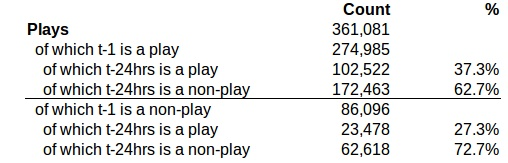
\includegraphics[width=7cm, keepaspectratio,]{fig012b.jpg}
	\caption{}
	\label{fig12b}
\end{figure} 

What both of these results tell us is that fairly high precision score of around 76\% ought ot be possible purely based on t-1 but going above this while having a good precision score on the non-play events will be harder.

Finally it was found that of rows where all timelags had a non-play event, 0.62\% of rows had a play event. As this was a low number it was deemed safe to remove all such rows from the dataset in order to improve the speed and quality of analysis. 

\subsection{Outliers}

The data was checked for any unusual outliers that may impinge upon the goal of developing a model to predict user behaviour. An analysis of plays by user reveals a high amount of variance between users on how many tracks are played. 

\begin{figure}[h!]
	\centering
	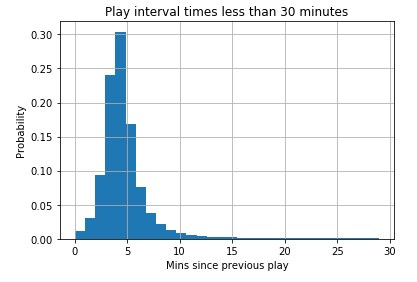
\includegraphics[width=7cm, keepaspectratio,]{fig003.jpg}
	\caption{}
	\label{3d}
\end{figure} 

For our purposes these are include as evidence that the user was interested in playing music at time $t$.

We can also assume that the song plays are not independent of one another, in that the probability of a play event at time t+1 is significantly higher if there was an event at time t. 


\subsection{Outliers}

The data was checked for any unusual outliers that may impinge upon the goal of developing a model to predict user behaviour. An analysis of plays by user reveals a high amount of variance between users on how many tracks are played. 

\begin{figure}[h!]
	\centering
	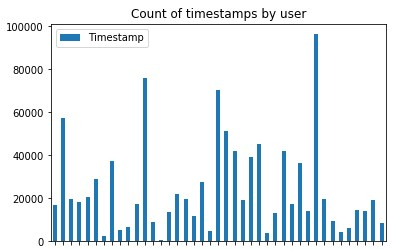
\includegraphics[width=7cm, keepaspectratio,]{fig002.jpg}
	\caption{Total play count by user}
	\label{fig2}
\end{figure} 


\newpage

Further analysis showed one user in particular with very high amount of plays, with very low durations, suggesting it was likely to have been generated by a bot, possibly a LastFM test. This was excluded from the dataset.

\section{Main results} % Methodology

Fig. \ref{fig13a} shows the results from our experiments. We see how our baseline model scores highly on accuracy but low on recall. In other words as a sequencce of plays often appear together in batches, assuming $t = t-1$ is often correct, but it fails to pick up the start and end points of a song.

\begin{figure}[h!]
	\centering
	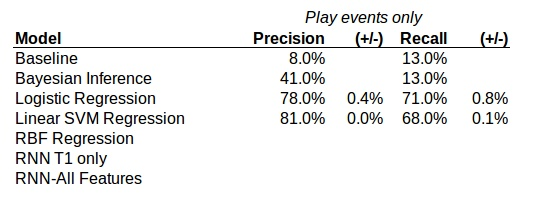
\includegraphics[width=8cm, keepaspectratio,]{fig013b.jpg}
	\caption{}
	\label{fig13b}
\end{figure}  


The Bayesian Inference model performs poorly on both measures. This would suggest that the difference between the population patterns and what is observed at an individual level is too large.

Our remaining models exhibit the tension between achieving a good accuracy and achieving a good recall.
The Logistic regression model performs below average on precision but is second highest on recall. The Linear SVM and RMF regression models are on par with one another with the former achieving the highest score on prevision, and the latter on recall. 

The Linear SVM model ignores probabilities that fall within a margin of the decision boundary during its optimization process. That this translates into performing well on precision may be due to placing lesser emphasis on ad-hoc play events that aren't indicative of a users general behaviour, as these probablities would likely fall near the decision boundary. Alternatively it could be better at dealing with the first play of a sequence whereby if often, but not always occurs at the same time each day; again leading to probabilities nearer the decision boundary.

The RBF model generally performs well on both metrics. Note that the RBF classifciation was restricted to 100k rows of training data as it was found the computational cost of 500k rows was too high so it had less training data to work with than the Linear SVM. The high recall rate of 68\% indicates that inputs have a non-linear relationship to the output and that this is especially helpful to predicting the start and end of a play sequence as seen by the high recall score. 
 
The RNN models were trained on 50k rows of data due to the computational cost of evaluating a large number of hyperparameters. Given the much smaller training set the results we obsertve are better than expected.  The final parameters for the models were a 250 units, 4 LSTM layers, and a class-weghting of 2.0 for play events.

\section{Important features}
The advantage of logistic regression and linesr SVM models are that it is easy to interpret the co-efficients used. The coefficients in a lgostic regression modle are an indicator of the strength of that feature in determining the output, while the coefficient in a linear SVM are an indicator of that feature in determining the decision boundary.

Fig XXX shows the co-efficients from both models. We see that t-1 was by far the most important feature. This is expcted and it's importance crowds out the other features. Re-running both models with only T1 gave us 

\section{RNN Hyper parameter tuning}

The advantage of the RNN model is that it determines the features by itself. However this comes at a prices with many more hyperparamters to tune, requiring a lot more time.

For our research the dataset was reduced in order to perform the desired number of hyperparameter tests. The number of hidden layers, units, timeteps, samples, and iterations all played a singificant part in impacting the time of a single run. 

Fig XXX shows the results of some of the other tests that were performed.

From this we see that XXX

\begin{figure}[h!]
	\centering
	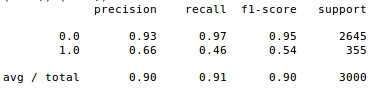
\includegraphics[width=7cm, keepaspectratio,]{fig011.jpg}
	\caption{}
	\label{fig:fig11}
\end{figure} 



% Chapter 5

\chapter{Summary} % Main chapter title

\label{Chapter6} 

\section{Conclusion}

Predicting the propensity of a user to listen to music at a certain time, based on their recent listening history can be applied to a range of other areas such as the propensity to purchase, electricity usage, or the demands on a public transport system. In all these a good modeling of the temporal patterns helps with prediction.

Within the literature modeling the problem as a temporal point process is one of the most common methods and this research did likewise in several of the machine learning algorithms that were evaluted.

As music listening is typically long periods of non-play events, followed by sequential periods of play events, the problem becomes one of a balance between precision and recall. Improving recall requires predicting the start and end of a sequence while precision favours restricting predictions to when $t-1 = 1$. This effect is seen in our baseline model which scored 79\% on precision and 13\% on recall after 5-fold cross validation.

It is also seen in the linear SVM models which is less impacted by cases that fall close to the decision boundary as the start of and end of a sequence are likely to be.

From a practical perspective, predicting the start and end of series of events is what is of most interest. In this respect it seems non-linear models may perform better than linear ones with the RBF model achieving a 76\% recall score (while maintaining a high 77\% precision score), and the the RNN-LSTM model achiving 69\% and 70\% respectively.

\section{Future research}

Future research into the matter temporal point proceses should investigate whether non-linear models are indeed better at detecting both the start of an event process as well as noiser data in which the patterns may not be as obvious.

If non-linear models perform better at these problems, then, given the performance of RNN-LSTM models on a small set of data, they may be prove to perform exceptionally well in learning to model such temporal patterns with larger amounts of data and training. Currently the training time on an average laptop proved to be a bottleneck but with processing speeds constantly improving we may be entering an age where such models become practical in the commercial data science field. 

Finally the research touched upon (see Appndices) but not fully investigated the time it takes for models to adapt to new users. Hybrid models or advanced Bayesian models, that balance the observations coming from the user with wider prior knowlege, may be the key to learning the behaviour of individuals. After all the best predictor for a users behaviour, is observing the user themselves.

%----------------------------------------------------------------------------------------
%	THESIS CONTENT - APPENDICES
%----------------------------------------------------------------------------------------

\appendix % Cue to tell LaTeX that the following "chapters" are Appendices

% Include the appendices of the thesis as separate files from the Appendices folder
% Uncomment the lines as you write the Appendices

% Appendix A

\chapter{Appendices}

\section{A. Further detail of experiments}

\section{Bayesian Inference}

Prior probabilities were calculated or each half-hourly period in a week. Fig \ref{fig10b} shows the calculations for the first 2.5 hours of a Sunday (d-hour-hh format). 

Our parameter of interest is the mean for the Beta distribution representing the probability of play in that time period. We estimate this by calculating probability of a play (total plays in period / count of plays and non-plays) per user, then taking the mean and variance across users. $a$ and $b$ are then determined as:
$a = (\frac{(1- \mu)}{\sigma} - \frac{1}{\mu}) \mu^2$
and
$\beta=\alpha\left(\frac{1}{\mu}-1\right)$.

\begin{figure}[h!]
	\centering
	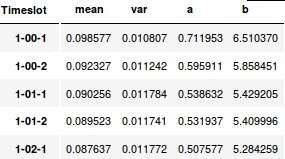
\includegraphics[width=4cm, keepaspectratio,]{fig010b.jpg}
	\caption{}
	\label{fig10b}
\end{figure} 

This allows us to visualize the prior probability for any given time period as shown in \ref{fig10c}.

\begin{figure}[h!]
	\centering
	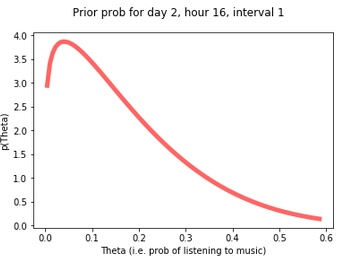
\includegraphics[width=5cm, keepaspectratio,]{fig010c.jpg}
	\caption{}
	\label{fig10c}
\end{figure} 

Once established we can calculate the liklihood of an individual user listening to music in a given time period by passing their observations as they come in for a specific timeslot $s$: $(H_{t,s})$ , into a Beta-Binomial formula to determine the probability of listening at the next occurence of that time slot as shown in <TBC>

Finally the threshold at which we determine that a probability constitutes a Play event is determined by comparing the false positive rates with the true positive rates using a ROC curve (\ref{fig10d}). This tells us that 0.4 is the optimal threshold at which to determine a Play event.

\begin{figure}[h!]
	\centering
	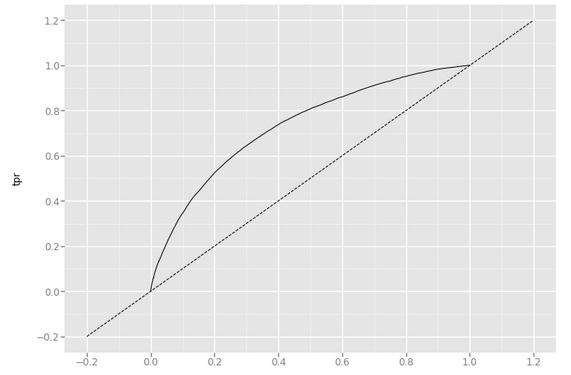
\includegraphics[width=5cm, keepaspectratio,]{fig010d.jpg}
	\caption{ROC curve showing 0.4 as the optimal threshold}
	\label{fig10d}
\end{figure} 

The results from the model are shown in figure \ref{fig10e}. We see that the recall and precision of play events (as denoted by 1) is very low suggesting that relying on a Bayesian approach centered around a weekly profile of each users habits is not an effective method for predicting a play event for a new time period.

\begin{figure}[h!]
	\centering
	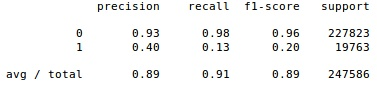
\includegraphics[width=7cm, keepaspectratio,]{fig010e.jpg}
	\caption{Beta-Bionmial Model Results}
	\label{fig10e}
\end{figure} 

\section{Feature analysis}

An advantage of logistic regression over non-linear models is that the coefficients are easily interpretable. While featuer engoneering was not the focus of this research an examination of these can yield insight into which features may be unecessary. 

\begin{figure}[h!]
	\centering
	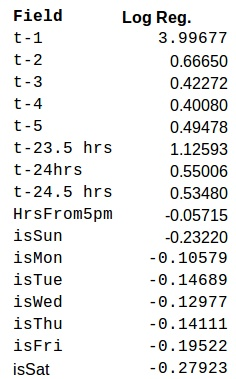
\includegraphics[width=4cm, keepaspectratio,]{fig014.jpg}
	\caption{}
	\label{fig14}
\end{figure} 

Fig \ref{fig14} shows that $t-1$ was by far the most important feature. This is expcted and it's importance crowds out the other features. Interestingly the t-24 hour period appears to have a stronger influence than $t-2$ to $t-5$ once $t-1$ has been accounted for. This reflects the daily patterns we observed in the preliminary analysis. The days of the week also pick up on the fact that weekeneds are somewhat different to weekdays thereby offering one area where the model could be simplified. Finally the hours from 5pm have a very small impact, and is likely unecessary if $t-24hrs$ is also used

\section{RNN Hyper parameter tuning}

For our evaluation of the RNN-LSTM model the dataset was reduced in order to perform the desired number of hyperparameter tests. It was found that the number of hidden layers, units, timeteps, samples, and iterations all played a signficant part in impacting the time it took to train the model. Typical run times were several hours long. 

Fig \ref{fig15} shows the results of some of the other tests that were performed. The improvment in performance comes with an increased in hidden layers, although this also leads to longer training times.

\begin{figure}[h!]
	\centering
	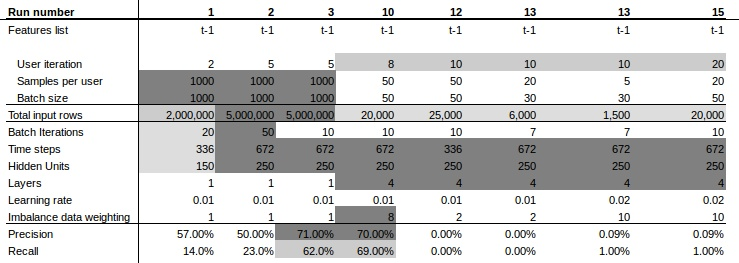
\includegraphics[width=7cm, keepaspectratio,]{fig015.jpg}
	\caption{}
	\label{fig15}
\end{figure}

\section{Adaptability to new users}

We also looked at the performance of models when it comes to learning the patterns of new users. Tie figures below show how the accuracy stablizied over time for each of the 10 test users. The periods indicate half-hourly intervals with 2-3,000 periods (1.5-2 months) appearing to be the time it takses to learn the habits of a typical user. 
\begin{figure}[h!]
	\centering
	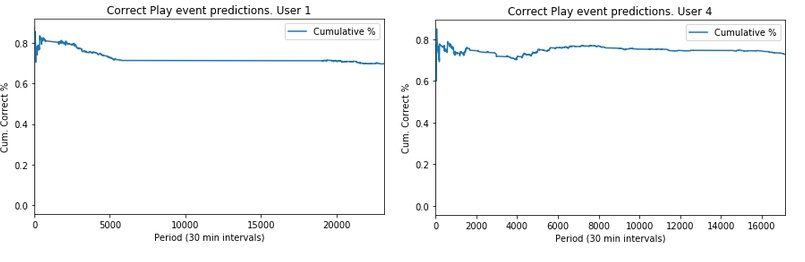
\includegraphics[width=7cm, keepaspectratio,]{fig008a.jpg}
	\caption{}
	\label{fig:fig8a}
\end{figure} 

\begin{figure}[h!]
	\centering
	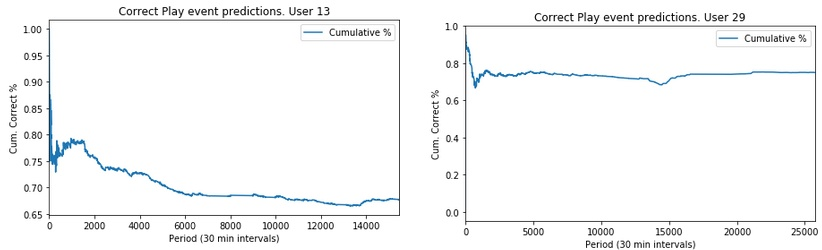
\includegraphics[width=7cm, keepaspectratio,]{fig008b.jpg}
	\caption{}
	\label{fig:fig8b}
\end{figure} 

\begin{figure}[h!]
	\centering
	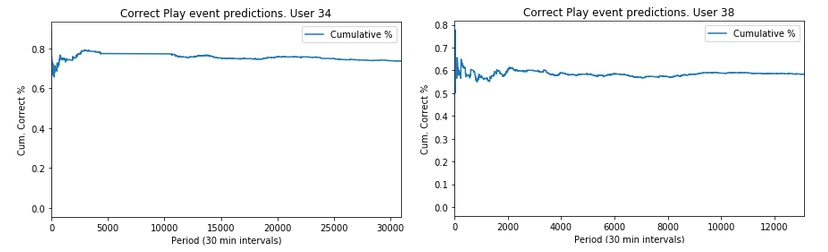
\includegraphics[width=7cm, keepaspectratio,]{fig008c.jpg}
	\caption{}
	\label{fig:fig8c}
\end{figure} 

\begin{figure}[h!]
	\centering
	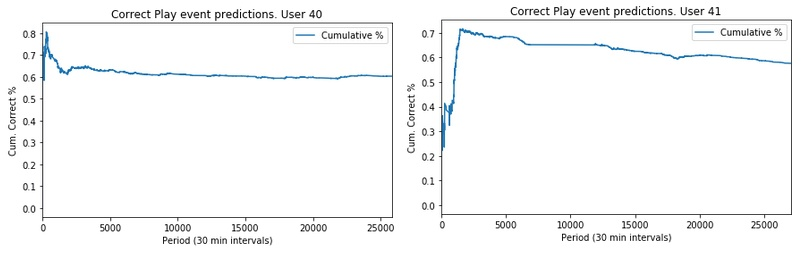
\includegraphics[width=7cm, keepaspectratio,]{fig008d.jpg}
	\caption{}
	\label{fig:fig8d}
\end{figure} 

\begin{figure}[h!]
	\centering
	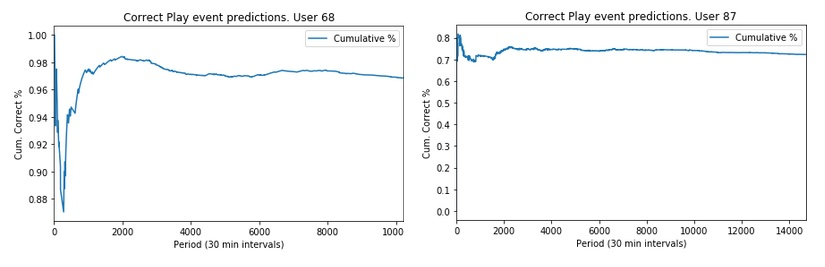
\includegraphics[width=7cm, keepaspectratio,]{fig008e.jpg}
	\caption{}
	\label{fig:fig8e}
\end{figure} 


From these charts it appears that two months worth of data is required to for the model to rget trained up on a new user.


\section{Content not used} % Main appendix title

Intro:
At an aggregate level, behaviour may appear to be deterministic, such as the times at which peak rush-hour occurs, but such behaviour is often composed of thousands or millions of individual stochastic processes such as the decisions made by individuals as to whether to leave work at 5pm or continue working a little longer.

While the modeling of aggregate patterns is well understood, these models ofen breakdown when applied to customizing results for individual users. At this level the temporal patterns of an individual combined with the behaviour of the population may be a better predictor of event timing. For instance, sticking with the example above, the times at which a person has lunch during the day may help predict that they will finish work a little later.


%\include{Appendices/AppendixB}
%\include{Appendices/AppendixC}

%----------------------------------------------------------------------------------------
%	BIBLIOGRAPHY
%----------------------------------------------------------------------------------------
\printbibliography[heading=bibintoc]

%----------------------------------------------------------------------------------------

\end{document}  
